\section{Results}
\label{sec:results}

\subsection{Does the pretrained encoder beat a random one?}
\label{sec:results_main}

Table~\ref{tab:main} reports the main comparison on the full 66-channel input. Both embedding
arms are far above the permutation null (null mean $0.332$, 95th percentile $0.364$;
$p < 0.01$ for both), so the task is decodable and the pipeline is sound.

\begin{table}[t]
\centering
\caption{Main comparison (all 33 pairs, 17 leave-one-subject-out folds, 64 matched dimensions).
Chance is 0.333. CIs are bootstrap 95\,\% intervals over folds for the difference.}
\label{tab:main}
\begin{tabular}{lccc}
\toprule
Arm & LOSO accuracy & $\Delta$ vs pretrained & paired $p$ (95\,\% CI) \\
\midrule
MtReNIRS (pretrained) & $\mathbf{0.4686 \pm 0.0955}$ & --- & --- \\
Random-init, mean of 10 seeds & $0.4482 \pm 0.0102$ & $+2.04$ pp & $0.188$\;[$-0.82$, $+4.86$] \\
Classical features & $0.4098 \pm 0.0754$ & $+5.88$ pp & $0.014$\;[$+1.86$, $+10.00$] \\
\bottomrule
\end{tabular}
\end{table}

The pretrained encoder is numerically the best arm, but \textbf{its advantage over a randomly
initialised encoder of the same architecture is $+2.04$~pp and not statistically significant}
($p = 0.188$; Wilcoxon $p = 0.225$; 95\,\% CI $[-0.82, +4.86]$ pp). The ten random seeds are
tightly clustered ($0.4482 \pm 0.0102$, range $0.4353$--$0.4696$), so this is not seed noise; the
pretrained model sits at the top of that distribution but the sample of 17 folds cannot resolve
the difference.

By contrast, the architecture does significantly outperform hand-crafted features
($+5.88$~pp, $p = 0.014$), and the random encoder alone also beats classical features
($+3.84$~pp, $p = 0.039$). The reading we take is that \emph{the spatial--temporal transformer
representation}, not the pretraining, supplies most of the measurable benefit on this task.

\begin{figure}[t]
\centering
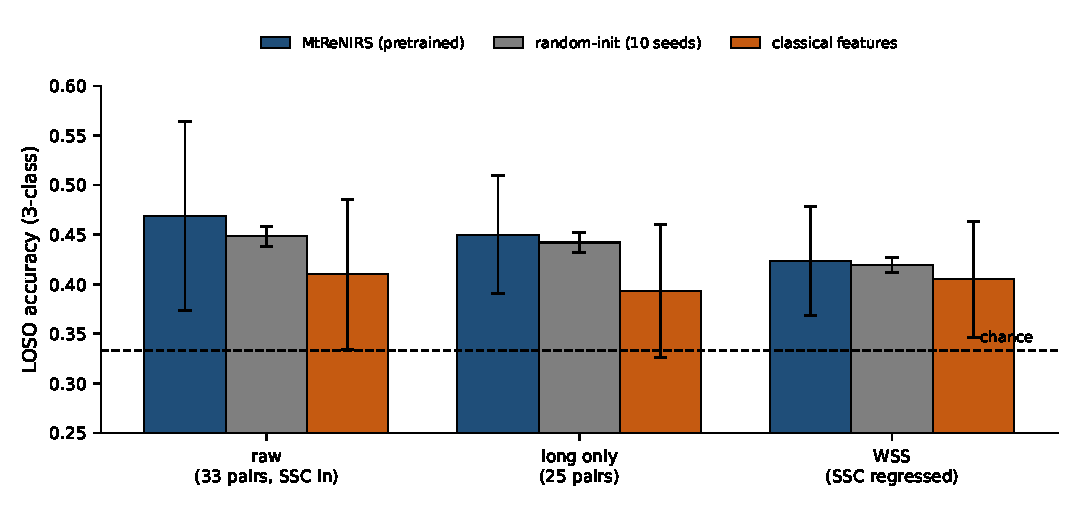
\includegraphics[width=\linewidth]{figures/fig_arms.pdf}
\caption{Leave-one-subject-out accuracy by arm and preprocessing variant. Error bars are standard
deviations over folds; the dashed line is chance. Removing short-separation channels and, more
strongly, regressing them out reduces accuracy and compresses the differences between arms.}
\label{fig:arms}
\end{figure}

\subsection{Short-separation regression reduces decoding accuracy}
\label{sec:results_wss}

Table~\ref{tab:variants} and Figure~\ref{fig:arms} report the preprocessing ablation. Dropping the
eight short-separation channels from the model input costs $1.86$~pp (pretrained arm,
$p = 0.318$), and additionally regressing their contribution out of the long channels costs a
further $2.65$~pp, for a total of $4.51$~pp between \emph{raw} and \emph{wss}
($p = 0.102$). Individually these differences are not significant at 17 folds, but the ordering
is consistent in every arm and the pattern is monotone.

\begin{table}[t]
\centering
\caption{Preprocessing ablation. WSS = short-separation channels regressed out of long channels
before epoching. Each column is the same ten-seed and classical comparison as
Table~\ref{tab:main}.}
\label{tab:variants}
\small
\begin{tabular}{lccccc}
\toprule
Variant & Pretrained & Random (10 seeds) & Classical & Pre.\ $-$ rand. & Pre.\ $-$ class. \\
\midrule
raw (33 pairs)      & $\mathbf{0.4686}$ & $0.4482$ & $0.4098$ & $+2.04$ ($p{=}0.19$) & $+5.88$ ($p{=}0.014$) \\
long only (25)      & $0.4500$ & $0.4421$ & $0.3931$ & $+0.79$ ($p{=}0.41$) & $+5.69$ ($p{=}0.006$) \\
wss (25, regressed) & $0.4235$ & $0.4192$ & $0.4049$ & $+0.43$ ($p{=}0.71$) & $+1.86$ ($p{=}0.30$) \\
\bottomrule
\end{tabular}
\end{table}

Two features of this ablation matter. First, the \emph{architecture} advantage over classical
features is significant before cleaning ($p = 0.014$ and $p = 0.006$) and disappears after
cleaning ($p = 0.297$). Second, the accuracy of the classical arm is essentially unaffected by
the same manipulation ($0.4098 \to 0.3931 \to 0.4049$). The manipulation therefore does not
simply remove noise from all arms equally: it preferentially removes information that the
embedding arms were using.

We interpret this as evidence that a component of the decodable signal in this paradigm is
\emph{systemic} rather than cortical, consistent with the warning of \citet{rybar2024cue} that
non-neural structure can inflate decoding. If that reading is correct, short-separation
regression does what it is designed to do---and in doing so removes signal, not only noise, when
the task is accompanied by global physiological changes that differ between conditions. We treat
this as a cautionary result rather than a refutation of the method: it is one paradigm, one
dataset, and the contrasts are individually below significance.

\subsection{Naive feature stacking significantly degrades performance}
\label{sec:results_stack}

At matched total dimensionality, concatenating encoder and classical features is
\emph{worse} than the encoder alone (Table~\ref{tab:stack}): $-4.71$~pp, $p = 0.042$, 95\,\% CI
$[-8.73, -0.59]$. The stack is statistically indistinguishable from classical features alone
($+1.18$~pp, $p = 0.567$), and the same pattern holds for the random-init arm
($-2.75$~pp, $p = 0.023$).

\begin{table}[t]
\centering
\caption{Feature-bank stacking at matched dimensionality (raw variant).}
\label{tab:stack}
\begin{tabular}{lcc}
\toprule
Arm & LOSO accuracy & Comparison \\
\midrule
Pretrained (PCA-64) & $\mathbf{0.4686 \pm 0.0955}$ & --- \\
Stack: pretrained + classical (32+32) & $0.4216 \pm 0.0626$ & $-4.71$ pp vs pre., $p=0.042$ \\
Classical alone & $0.4098 \pm 0.0754$ & stack $-1.18$ pp, $p=0.567$ \\
\bottomrule
\end{tabular}
\end{table}

The per-channel mean and slope features are therefore largely redundant with the transformer
embeddings: forcing half the dimensions to carry them costs more information than they add. Any
integration of multiple representations for fNIRS should be \emph{learned}---attention or gating
over feature banks, or joint training with a shared trunk---rather than concatenated.

\subsection{Companion tool: detectability as a pre-study check}
\label{sec:results_tool}

Figure~\ref{fig:detect} illustrates the calculator on two informal, self-collected
trigger-free pilot sessions (16 long channels, 50~Hz, natural-image viewing, no hardware
triggers recorded; see \S\ref{sec:methods_tool} for provenance and release decision). Injecting synthetic responses at the nominal design's onsets yields a detection floor
of $0.24$~$\mu$M peak HbO for Session~A and $0.35$~$\mu$M for Session~B at 80\,\% power.
On the real data, no stimulus-locked structure was recovered: the maximum template correlation
was $0.139$ and $0.140$, against phase-randomised null means of $0.145$ and $0.139$
($p = 0.58$ and $0.50$); a free-period search over 20--45~s gave $p = 0.14$--$0.87$; and three
unsupervised segmenters recovered no protocol-like structure. The design could thus have
detected a strong response but not a weak one, and---because the onsets were never recorded---the
dataset cannot support stimulus-locked analysis regardless. We report this because it is exactly
the judgement we would want a reviewer to demand of a decoding claim, and because the same tool
converts a vague worry about statistical power into a number a study can be designed against.

\begin{figure}[t]
\centering
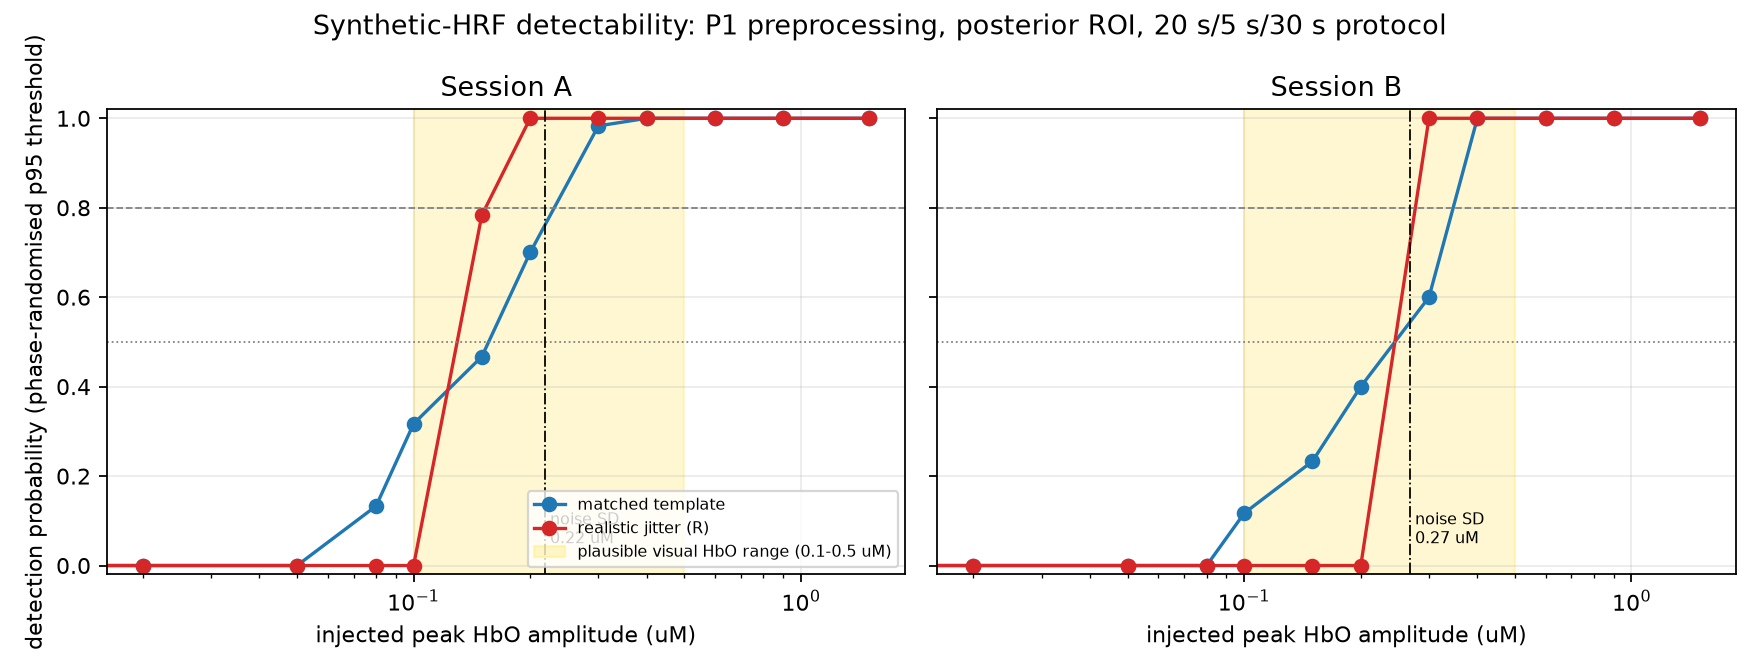
\includegraphics[width=\linewidth]{figures/fig_detectability.png}
\caption{Detectability curves for the two participants of a trigger-free recording. Shaded band:
plausible visual-cortex HbO range. The curve gives the probability that a synthetic response of a
given amplitude, injected at the hypothesised onsets, would be recovered by the same pipeline
applied to the real data.}
\label{fig:detect}
\end{figure}
